\begin{center}
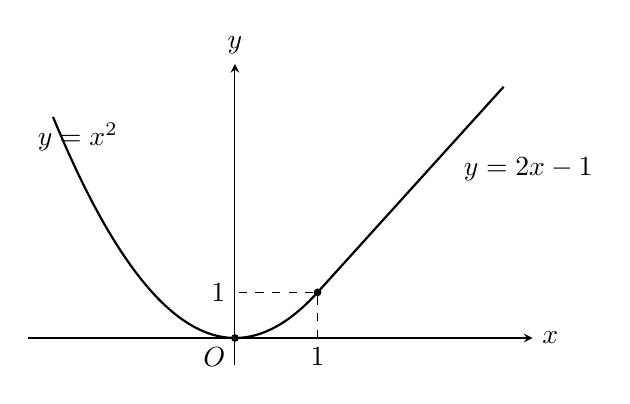
\begin{tikzpicture}[x=1.05cm,y=.58cm,>=stealth]
\draw[->](-2.5,0)--(3.6,0)node[right]{$x$};
\draw[->](0,-.6)--(0,6)node[above]{$y$};
\draw[thick,domain=-2.2:1,samples=70,smooth]plot(\x,{\x*\x});
\draw[thick](1,1)--(3.25,5.5);
\draw[dashed](1,0)--(1,1)--(0,1);
\fill(0,0)circle(1.4pt);
\fill(1,1)circle(1.4pt);
\node[below left]at(0,0){$O$};
\node[below]at(1,0){$1$};
\node[left]at(0,1){$1$};
\node at(-1.9,4.4){$y=x^2$};
\node[right]at(2.65,3.7){$y=2x-1$};
\end{tikzpicture}
\captionof{figure}{在连接点连续衔接的二次函数与一次函数}
\label{sol:fig:functions-piecewise}
\end{center}
